\chapter{Anexo A: Manual de instalación}

A continuación se detallan los pasos a seguir para el despliegue del sistema de video-vigilancia inteligente. Para la instalación general es necesario tener instalado en el equipo los siguientes paquetes de software:

\begin{enumerate}
    \item Python (Version 3.7 o posterior).
    \item venv (Manejador de entornos virtuales)
    \item git (Controlador de versiones)
    \item pip (Manejador de paquetes de python) 
\end{enumerate}

Por otra parte, el dispositivo donde se realizará la instalación debe contar con una conexión a la red de internet.

\section*{Módulo de cámaras}
Este módulo puede ser instalado en un computador (laptop o de escritorio) como también en un dispositivo RaspberryPi, el cual debe tener previamente instalados los paquetes requeridos anteriormente descritos. Este módulo permite la conexión de una cámara web (integrada o individual) al servidor del sistema de video-vigilancia, por lo que es necesario contar con una.\\

Para realizar la instalación del módulo de cámaras se siguen los siguientes pasos:

\begin{enumerate}
    \item Descargar el código fuente de la aplicación desde el enlace: \begin{center}
        \url{https://github.com/srodrigo23/security-camera.git}
    \end{center}
    \item En el directorio de la carpeta de descarga, se debe crear el entorno virtual del módulo por medio del siguiente comando: 
    \begin{center}
        \shellcmd{python3 -m venv .venv}    
    \end{center}
    \item Instalar las depencias del módulo por medio del comando:
    \begin{center}
        \shellcmd{pip install -r requirements.txt}
    \end{center} 
    \item Una vez instaladas las depencias solo queda lanzar la ejecución del módulo por medio del comando:\begin{center}
        \shellcmd{./run.sh}
    \end{center}
\end{enumerate}

Una vez completados los pasos se carga la vista del módulo de cámaras, listo para su conexión con el servidor.

\begin{figure}[H]
    \begin{center}
        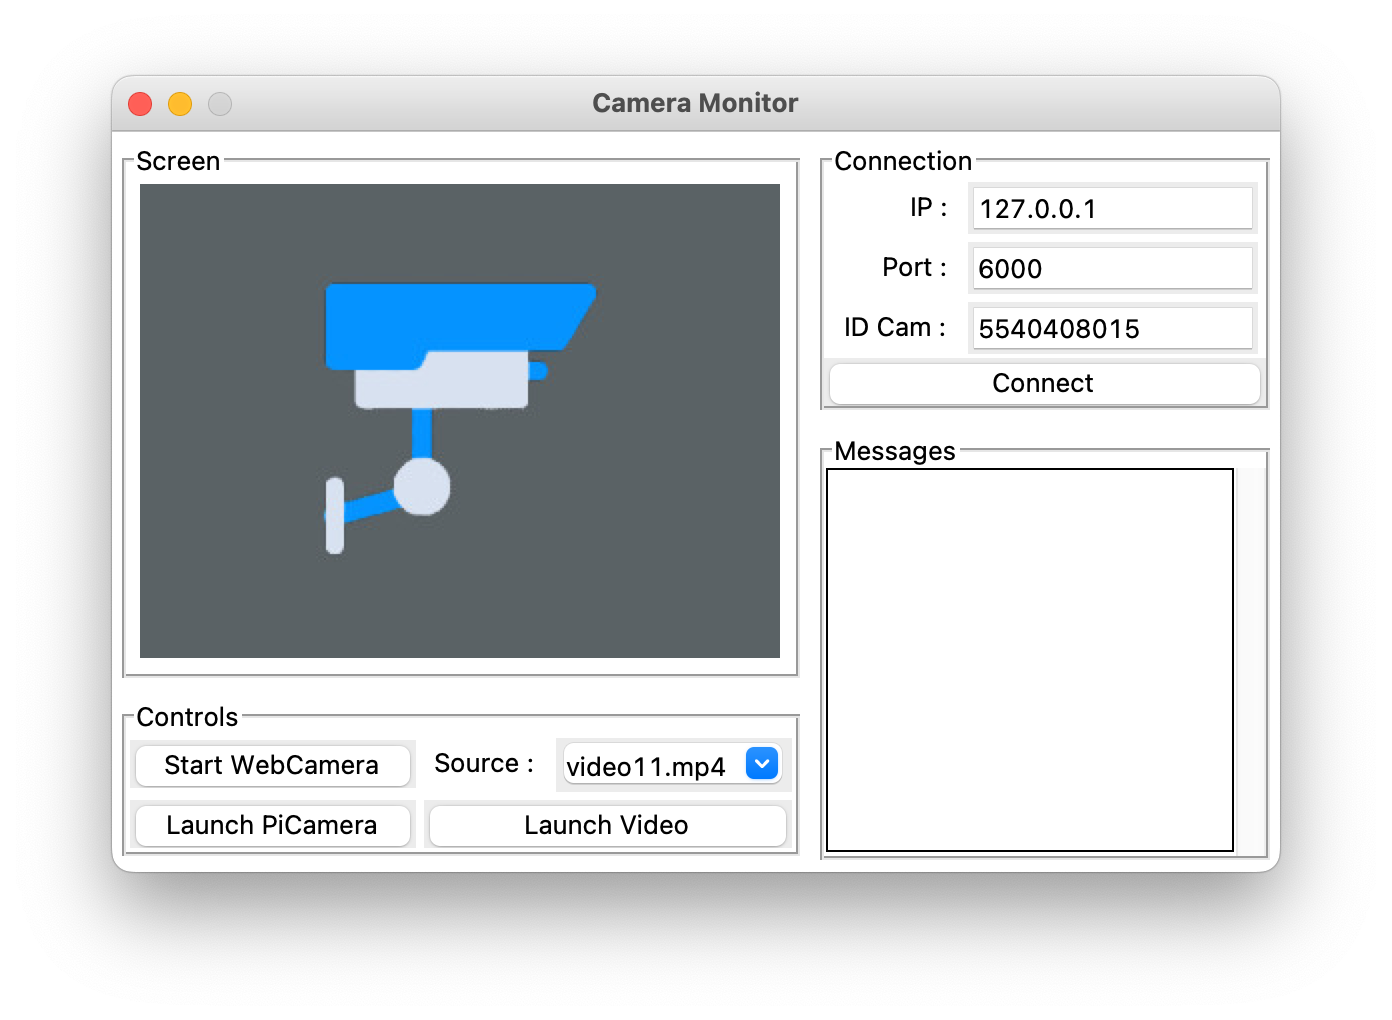
\includegraphics[width=13cm]{img/anexos/mod_camera.png}
        \caption{Interfaz del módulo de cámaras.}
        Fuente : Elaboración propia
    \end{center}
\end{figure}

\section*{Módulo de servidor}
El módulo de servidor consta de dos sub-módulos: servidor-TCP y el servidor-WEB. Ambos son relevantes para el sistema de video-vigilancia, por lo cual deben estar correctamente instalados para una correcta ejecución del sistema.
\subsection*{Servidor TCP}
Este módulo puede ser instalado en un computador (laptop o de escritorio). Durante su ejecución espera nuevas conexiones del módulo de cámaras, para gestionar la transmisión de fotogramas, realizar las detecciones y mandar las notificaciones.\\

Para realizar la instalación del módulo del servidor-TCP se siguen los siguientes pasos:
\begin{enumerate}
    \item Descargar el código fuente de la aplicación desde el enlace: \begin{center}
        \url{https://github.com/srodrigo23/security-system-server.git}
    \end{center}
    \item En el directorio de la carpeta de descarga, se debe crear el entorno virtual del módulo por medio del siguiente comando: 
    \begin{center}
        \shellcmd{python3 -m venv .venv}    
    \end{center}
    \item Instalar las depencias del módulo por medio del comando:
    \begin{center}
        \shellcmd{pip install -r requirements.txt}
    \end{center} 
    \item Una vez instaladas las depencias solo queda lanzar la ejecución del módulo por medio del comando:\begin{center}
        \shellcmd{./run.sh}
    \end{center}
\end{enumerate}

Una vez completados los pasos se carga la interfaz de consola del servidor-TCP, listo para recibir conexiones de cámaras.

\begin{figure}[H]
    \begin{center}
        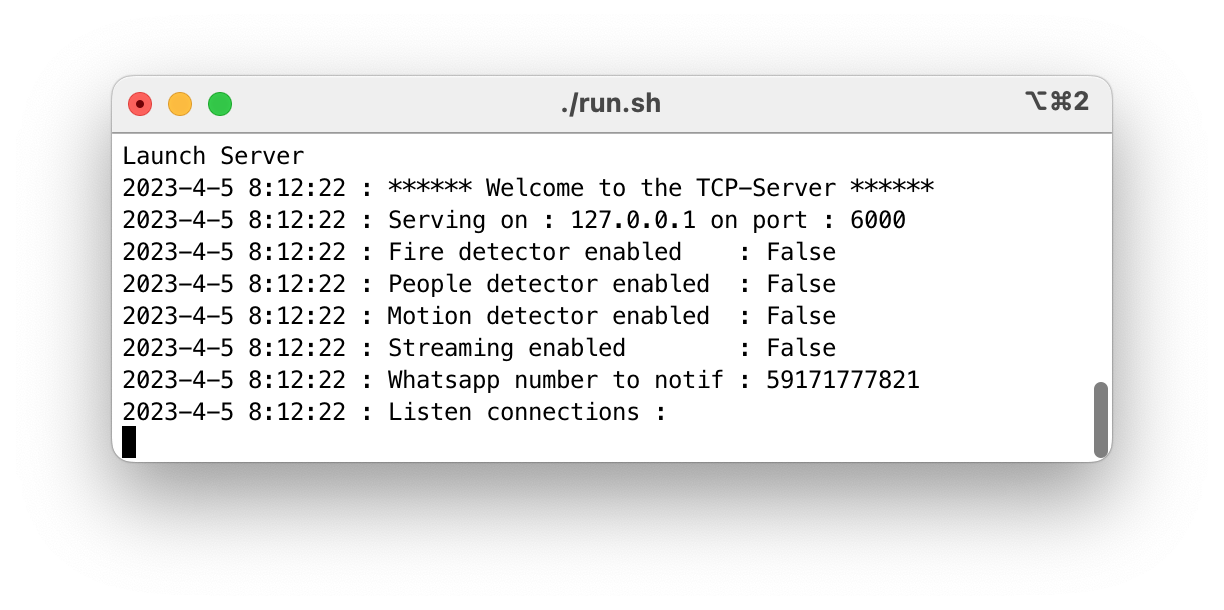
\includegraphics[width=13cm]{img/anexos/mod_tcp.png}
        \caption{Interfaz de consola del servidor TCP.}
        Fuente : Elaboración propia
    \end{center}
\end{figure}
\subsection*{Servidor web}

Este módulo puede ser instalado en un computador (laptop o de escritorio) como también en un dispositivo RaspberryPi, el cual debe tener previamente instalados los paquetes requeridos anteriormente descritos. Este gestionar las solicitudes HTTP que provienen desde un reprodicutor web de video adaptativo permitiendo asi la transmisión de video en vivo.\\

Para realizar la instalación del servidor web se deben seguir los siguientes pasos:

\begin{enumerate}
    \item Descargar el código fuente de la aplicación desde el enlace: \begin{center}
        \url{https://github.com/srodrigo23/webserver.git}
    \end{center}
    \item En el directorio de la carpeta de descarga, se debe crear el entorno virtual del módulo por medio del siguiente comando: 
    \begin{center}
        \shellcmd{python3 -m venv .venv}    
    \end{center}
    \item Instalar las depencias del módulo por medio del comando:
    \begin{center}
        \shellcmd{pip install -r requirements.txt}
    \end{center} 
    \item Una vez instaladas las depencias solo queda lanzar la ejecución del módulo por medio del comando:\begin{center}
        \shellcmd{./run.sh}
    \end{center}
\end{enumerate}

Una vez completados los pasos se carga interfaz de consola del servidor-WEB, listo para atender todas las peticiones HTTP al servidor.

\begin{figure}[H]
    \begin{center}
        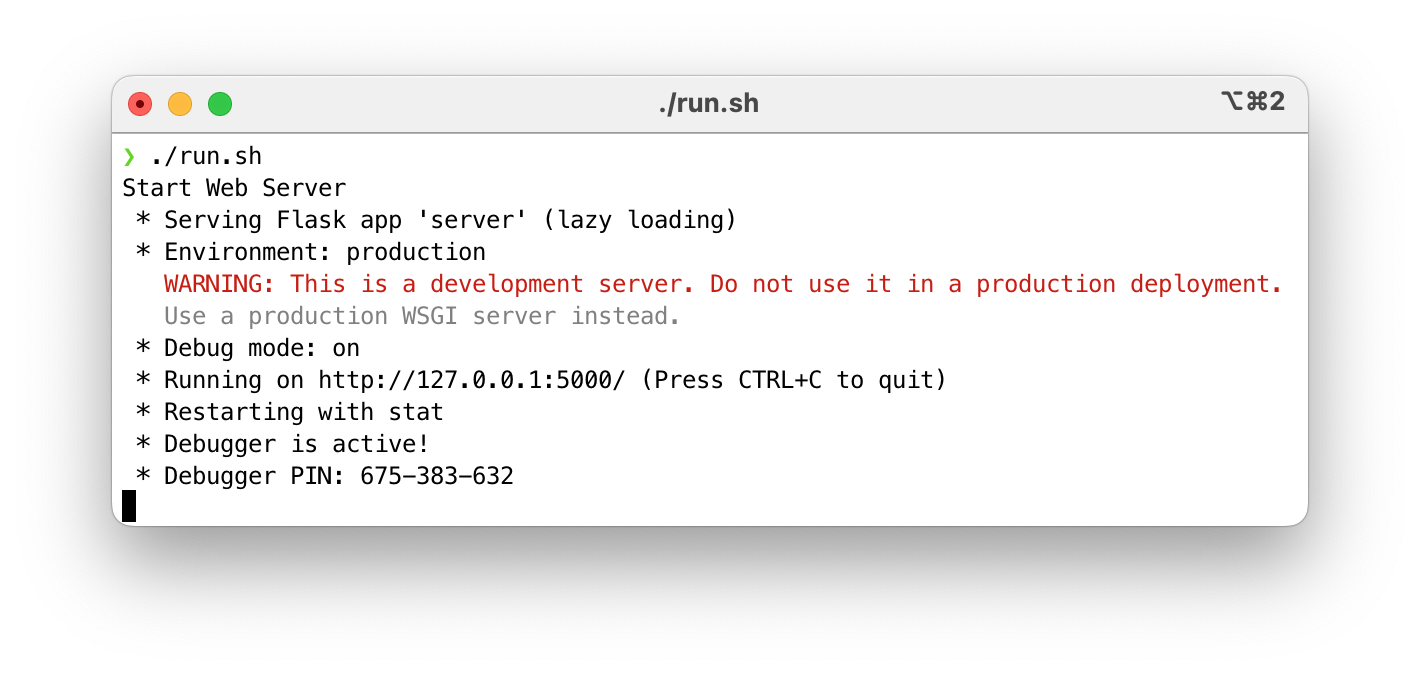
\includegraphics[width=13cm]{img/anexos/mod_web.png}
        \caption{Interfaz de consola del servidor Web.}
        Fuente : Elaboración propia
    \end{center}
\end{figure}
